% -----------------------------------------------
% Template for SMC 2019
% adaed from the template for SMC 2018
% -----------------------------------------------

\documentclass{article}
\usepackage{smc2019}
\usepackage{times}
\usepackage{ifpdf}
\usepackage[english]{babel}
\usepackage{cite}
\usepackage{physics}
%%%%%%%%%%%%%%%%%%%%%%%% Some useful packages %%%%%%%%%%%%%%%%%%%%%%%%%%%%%%%
%%%%%%%%%%%%%%%%%%%%%%%% See related documentation %%%%%%%%%%%%%%%%%%%%%%%%%%
\usepackage{amsmath} % popular packages from Am. Math. Soc. Please use the 
\usepackage{amssymb} % related math environments (split, subequation, cases,
\usepackage{amsfonts}% multline, etc.)
\usepackage{bm}      % Bold Math package, defines the command \bf{}
\usepackage[]{algorithm2e}
%\usepackage{paralist}% extended list environments
%%subfig.sty is the modern replacement for subfigure.sty. However, subfig.sty 
%%requires and automatically loads caption.sty which overrides class handling 
%%of captions. To prevent this problem, preload caption.sty with caption=false 
%\usepackage[caption=false]{caption}
%\usepackage[font=footnotesize]{subfig}


%user defined variables
\def\papertitle{Real-time Control of Advanced Physical Models using the Sensel Morph}
\def\firstauthor{Silvin Willemsen}
\def\secondauthor{Nikolaj Andersson }
\def\thirdauthor{Stefania Serafin}
\def\fourthauthor{Stefan Bilbao}

% adds the automatic
% Saves a lot of output space in PDF... after conversion with the distiller
% Delete if you cannot get PS fonts working on your system.

% pdf-tex settings: detect automatically if run by latex or pdflatex
\newif\ifpdf
\ifx\pdfoutput\relax
\else
   \ifcase\pdfoutput
      \pdffalse
   \else
      \pdftrue
\fi

\ifpdf % compiling with pdflatex
  \usepackage[pdftex,
    pdftitle={\papertitle},
    pdfauthor={\firstauthor, \secondauthor, \thirdauthor, \fourthauthor},
    bookmarksnumbered, % use section numbers with bookmarks
    pdfstartview=XYZ % start with zoom=100% instead of full screen; 
                     % especially useful if working with a big screen :-)
   ]{hyperref}
  %\pdfcompresslevel=9

  \usepackage[pdftex]{graphicx}
  % declare the path(s) where your graphic files are and their extensions so 
  %you won't have to specify these with every instance of \includegraphics
  \graphicspath{{./figures/}}
  \DeclareGraphicsExtensions{.pdf,.jpeg,.png,.eps}

  \usepackage[figure,table]{hypcap}

\else % compiling with latex
  \usepackage[dvips,
    bookmarksnumbered, % use section numbers with bookmarks
    pdfstartview=XYZ % start with zoom=100% instead of full screen
  ]{hyperref}  % hyperrefs are active in the pdf file after conversion

  \usepackage[dvips]{epsfig,graphicx}
  % declare the path(s) where your graphic files are and their extensions so 
  %you won't have to specify these with every instance of \includegraphics
  \graphicspath{{./LATEX/}}
  \DeclareGraphicsExtensions{.eps}

  \usepackage[figure,table]{hypcap}
\fi

%setup the hyperref package - make the links black without a surrounding frame
\hypersetup{
    colorlinks,%
    citecolor=black,%
    filecolor=black,%
    linkcolor=black,%
    urlcolor=black
}
\SetAlCapSkip{1em}

% Title.
% ------
\title{\papertitle}

% Authors
% Please note that submissions are NOT anonymous, therefore 
% authors' names have to be VISIBLE in your manuscript. 
%
% Single address
% To use with only one author or several with the same address
% ---------------
% \twoauthors
%   {Silvin Willemsen, Nikolaj Andersson and Stefania Serafin} { \\ Multisensory Experience Lab, CREATE, Aalborg University Copenhagen \\ %
%     {\tt \href{mailto:sil@create.aau.dk}{\{sil, nsa, sts\}@create.aau.dk}}}

% Two addresses
% --------------
\oneauthor
  {\firstauthor, \secondauthor and \thirdauthor} {Multisensory Experience Lab,\\
   Aalborg University Copenhagen \\
   Copenhagen, Denmark\\ %
    {\tt \href{mailto:sil@create.aau.dk}{\{sil, nsa, sts\}@create.aau.dk}}}

% Three addresses
% --------------
%   {\firstauthor} {{} %
%       {}}
%   {\secondauthor} {{Multisensory Experience Lab, CREATE, Aalborg University Copenhagen}
%      {\tt \href{mailto:sil@create.aau.dk}{\{sil, nsa, sts\}@create.aau.dk}}}
%   {\thirdauthor}{
%      {}}
    % {\fourthauthor} { Affiliation4 \\ %
    %  {\tt \href{mailto:author3@smcnetwork.org}{author3@smcnetwork.org}}}


% ***************************************** the document starts here ***************
\begin{document}
%
\capstartfalse
\maketitle
\capstarttrue
%
\begin{abstract}
Lorum Ipsum
\end{abstract}
%

\section{Introduction}\label{sec:introduction}
The behaviour of musical instruments can be well defined by partial differential equations (PDEs) \cite{Bilbao2018:Tutorial}.

Finite-difference schemes (FDSs)

The physical models (PMs) used as a case study in this project are the stiff string and the plate.

Used Modular Percussion Synthesis Environment (Bilbao) + On the limits of real-time physical modelling synthesis with a modular environment (Webb + Bilbao) as a basis and extended it to be interactive and used melodic rather than percussive components/elements.

On top of all this, we have used the expressive Sensel Morph \cite{sensel2018} control surface to control the PMs in real-time, something that to the best of the authors' knowledge has not been done before. 

This paper is structured as follows: Section \ref{sec:PDE} describes the PMs used in the implementation and Section \ref{sec:FDS} shows the FDSs used to digitally implement these models. Furthermore, Section \ref{sec:implementation} will show how to implement the FDSs, Section \ref{sec:instruments} shows several different configurations of PMs inspired by real musical instruments and finally Section \ref{sec:discussion} and Section \ref{sec:conclusion} will discuss and conclude upon the work shown in this paper.

\section{Models}\label{sec:PDE}
In this section, the partial differential equations for the damped stiff string and the plate will be presented. 

% \begin{equation}
%     \pdv[2]{u}{t} = \gamma^2 \pdv[2]{u}{x} -\kappa^2 \pdv[4]{u}{x} - 2\sigma_0\pdv{u}{t} + 2\sigma_1\frac{\partial^3u}{\partial tx^2}
% \end{equation}

\subsection{Stiff string}\label{subsec:stiffStringPDE}
The state $u = u(x,t)$ describes the transverse displacement of the string. The partial differential equation for the damped stiff string is defined as \cite{Bilbao2009:NumericalSoundSynthesis} 
\begin{equation}\label{eq:stiffString}
    u_{tt} = \gamma^2 u_{xx}-\kappa^2u_{xxxx} - 2\sigma_0u_{t} + 2\sigma_1u_{txx},
\end{equation}
where $\gamma$ is wave-speed with units of frequency [s$^{-1}$], $\kappa$ is a stiffness parameter
%[$\sqrt{\text{kg}}\cdot$m$^{-2}\cdot$ s$^{-2}$]
and $\sigma_0 \geq 0$ and $\sigma_1 \geq 0$ are frequency-dependent and frequency-independent damping respectively. The subscript for $u$ denotes a single derivative with respect to time $t$ or space $x$ respectively.


We can extend Equation \eqref{eq:stiffString} to a bowed string \cite{Bilbao2009:NumericalSoundSynthesis} 
\begin{align}
    \label{eq:bowedString} &u_{tt} = ... - \delta(x-x_\text{B})F_\text{B}\phi(v_\text{rel}), \quad \text{with} \\
    &v_\text{rel} = u_t(x_\text{B}) - v_\text{B}
\end{align}
%the $\delta$ function is only non-zero at the bowing point, effectively locating the bowing interaction.  
where $F_\text{B} = f_\text{B}/ M_\text{s}$ is the excitation function [m/s$^2$] with bowing force $f_\text{B}$ [N] and total string mass $M_\text{s}$ [kg]. The relative velocity $v_\text{rel}$ is defined as the difference between the velocity of the string at bowing point $x_\text{B}$ and the bowing velocity $v_\text{B}$ [m/s] and $\phi$ is a friction characteristic, which has been chosen to be \cite{Bilbao2009:NumericalSoundSynthesis}
\begin{equation}
    \phi(v_\text{rel}) = \sqrt{2a}v_\text{rel} e^{-av_\text{rel}^2+1/2}.
\end{equation}
Furthermore,
\begin{equation} \label{eq:dirac}
    \delta(x-x_\text{B}) =
\begin{cases}
    1, & \text{if } x=x_\text{B}\\
    0,              & \text{otherwise}
\end{cases}
\end{equation}
is referred to as the spatial Dirac delta function centered at $x_\text{B}$, which, when multiplied onto the excitation, applies it only to the point $x_\text{B}$ on the string.

Another, and more simple way to excite the string is by extending Equation \eqref{eq:stiffString} to
\begin{equation}
    \label{eq:excitedString} u_{tt} = ... + F_\text{e}E_\text{e},
\end{equation}
where excitation function $F_\text{e} = F_\text{e}(t)$ and distribution function $E_\text{e} = E_\text{e}(x)$. If the excitation is only applied to one point, the distribution function reduces to $\delta(x-x_\text{e})$.
\subsection{Plate}\label{subsec:platePDE}
In the case of a plate, the state $u = u(x,y,t)$ is now defined over two spatial dimensions. The PDE for a damped plate is \cite{Bilbao2009:NumericalSoundSynthesis}
\begin{equation}\label{eq:platePDE}
    u_{tt} = -\kappa^2 \Delta\Delta u - 2 \sigma_0 u_{t} + 2\sigma_1 \Delta u_{t},
\end{equation}
where $\kappa$ is again a stiffness parameter and $\Delta$ represents the 2D Laplacian.

\subsection{Connections}\label{sec:connections}
Adding connections between different PMs, further referred to as elements, adds another term to the string or plate equations
%% this paragraph is too wide for some reason
\begin{align}
    u_{tt} &= ... + F_\alpha E_\alpha, \\
    u_{tt} &= ... + F_\beta E_\beta,
\end{align}
where $F_\alpha$ and $F_\beta$ are the forces of the connection at connection areas $E_\alpha$ and $E_\beta$ respectively. If a connection area consists of only one point, $E$ reduces to a scaled version of $\delta(x-x_\text{c})$ where $x_\text{c}$ is the point of connection (see Equation \eqref{eq:excitationAreas}). We use the implementation as presented in \cite{Bilbao2009:ModularPercussion} where the connection between two elements is a non-linear spring. The forces it imposes on the elements it connects - denoted by $\alpha$ and $\beta$ - are defined as
\begin{subequations}\label{eq:connectionsPDE}
\begin{align}
    F_\alpha &= -\omega_0^2\eta - \omega_1^4\eta^3 - 2\sigma_\times\eta_t,\\
    F_\beta &= -\mathcal{M}_{\alpha/\beta}F_\alpha,
\end{align}
\end{subequations}
where $\omega_0$ and $\omega_1$ are the linear and non-linear spring coefficients respectively [N/m] %CORRECT??
, $\sigma_\times$ is a damping factor, $\mathcal{M}_{\alpha/\beta}$ is the mass ratio between the two elements and $\eta$ is the relative displacement between the connected elements at the point of connection. The subscript $t$ again denotes a derivative with respect to time.


\section{Finite-Difference Schemes}\label{sec:FDS}
To be able to digitally implement the continuous equations shown in the previous section, they need to be approximated. The models can be discretised at times $t = nk$, where $n \in \mathbb{N}$ and $k = 1 / f_\text{s}$ is the time-step with sample-rate $f_\text{s}$ and locations $x = lh$, where $l \in [0,N]$ with $N$ being the total number of points and $h$ is the grid-spacing of the model which is calculated differently for each model (see sub-sections below). The discretised variable $u_l^n$ is $u(x,t)$ at the $n$th time step and the $l$th point on the string. The plate is discretised using $x = lh$ where $l \in [0,N_x]$ with $N_x$ being the total horizontal number of points and $y = mh$ where $m \in [0,N_y]$ with $N_y$ being the total vertical number of points. 
Approximations for the derivatives in the equations found in Section \ref{sec:PDE} can be found in \cite{Bilbao2009:NumericalSoundSynthesis}. We will also use the notation for the difference and averaging operators found here. 

\textit{Note: In this paper we have used the simple case of a single point for bowing and connections. These can be extended to a bowing area or area of connection. For more information on this, we would like to refer the reader to \cite{Bilbao2009:ModularPercussion}}.

\subsection{Stiff String}\label{subsec:stiffStringFDS}
Equation \eqref{eq:stiffString} can be approximated using
\begin{equation}
\begin{aligned}\label{eq:stiffStringFDS}
\delta_{tt} u_l^n = &\gamma^2 \delta_{xx} u_l^n -\kappa^2\delta_{xx}\delta_{xx} u_l^n - 2\sigma_0\delta_{t\cdot} u_l^n  \\
&+ 2\sigma_1\delta_{t-}\delta_{xx}u_l^n.
\end{aligned}
\end{equation}
The extensions found in Equations \eqref{eq:bowedString} and \eqref{eq:excitedString} are approximated using
\begin{align}
    \delta_{tt} u_l^n &= ... - \delta_{x_\text{B}}F_\text{B}\phi(v_\text{rel}),\label{eq:bowedStringFDS}\\
    \delta_{tt} u_l^n &= ... + F_\text{e}E_\text{e},\label{eq:excitedStringFDS}
\end{align}
where $\delta_{x_\text{B}} = \delta(x-x_\text{B})$ (see Equation \eqref{eq:dirac}) and 
\begin{equation}\label{eq:descreteRelativeVel}
    v_\text{rel} = \delta_{t\cdot}u(x_\text{B})-v_\text{B}.
\end{equation}
For our implementation, clamped boundary conditions were used, defined as:
\begin{equation}\label{boundary}
    u = u_x = 0 \quad \text{where} \quad l = \{0, N\}.
\end{equation}
  
For stability reasons, the grid-spacing needs to abide the following condition
%section 7.2.3 numerical sound synthesis
\begin{equation}\label{eq:stabilityString}
    h \geq \sqrt{\frac{\gamma^2 k^2 + 4 \sigma_1 k + \sqrt {(\gamma^2 k^2 + 4 \sigma_1 k)^2 + 16 \kappa^2 k^2}}{2}}.
\end{equation}
The closer $h$ is to this limit, the higher the quality of the implementation. The number of points $N$ can then be calculated using 
\begin{equation}
    N = h^{-1}.
\end{equation}

\subsection{Plate}
Equation \eqref{eq:platePDE} can be approximated using
\begin{equation}
    \begin{aligned}\label{eq:plateFDS}
        \delta_{tt}u_{l,m}^n = &-\kappa^2 \delta_\Delta\delta_\Delta u_{l,m}^n - 2\sigma_0\delta_{t\cdot}u_{l,m}^n \\
        &+ 2\sigma_1\delta_{t-}\delta_\Delta u_{l,m}^n
    \end{aligned}
\end{equation}
As in the case of the stiff string, we chose to use clamped boundary conditions:
\begin{equation}
    \begin{aligned}
        u = u_x = 0 \quad &\text{where} \quad \: l \, \, = \{0, N_x\} \quad \text{and} \\
        u = u_y = 0 \quad &\text{where} \quad m = \{0, N_y\}
    \end{aligned}
\end{equation}
In the case of the plate, we set the number of horizontal and vertical points and calculate grid spacing $h$ from that using \cite{Bilbao2009:ModularPercussion}
\begin{equation}
    h = \frac{\sqrt{N_x / N_y}}{N_x}.
\end{equation}

\subsection{Connections}
The equations in \eqref{eq:connectionsPDE} can be approximated using \cite{Bilbao2009:ModularPercussion}
\begin{subequations}
\begin{align}\label{eq:connectionsFDS}
    F_\alpha &= -\omega_0^2\mu_{t\cdot}\eta - \omega_1^4\eta^2\mu_{t\cdot}\eta - 2\sigma_\times\delta_{t\cdot}\eta,\\
    F_\beta &= -\mathcal{M}_{\alpha/\beta}F_\alpha.
\end{align}
\end{subequations}
The relative displacement $\eta$ between $\alpha$ and $\beta$ can be calculated as
\begin{equation}
    \eta^n = h_\alpha u_{\alpha, x_{\text{c},\alpha}}^n - h_\beta u_{\beta,x_{\text{c},\beta}}^n,
\end{equation}
which, in other words, is the difference between the state of element $\alpha$ at connection point $x_{\text{c},\alpha}$ and the state of element $\beta$ at connection point $x_{\text{c},\beta}$ scaled by their respective grid-spacings $h_\alpha$ and $h_\beta$. Solving \eqref{eq:connectionsFDS} for $\eta^{n+1}$ yields
\begin{equation}
    \eta^{n+1} = p^nF_\alpha+r^n\eta^{n-1},
\end{equation}
with
\begin{subequations}
\begin{align}
    p^n &= \frac{-2}{2\sigma_x/k + \omega_0^2+\omega_1^4(\eta^n)^2},\\
    r^n &= \frac{2\sigma_x/k - \omega_0^2-\omega_1^4(\eta^n)^2}{2\sigma_x/k + \omega_0^2+\omega_1^4(\eta^n)^2}.
\end{align}
\end{subequations}
The (scaled) connection areas (simplified to be a single connection point) $E_{\alpha,\text{c}}$ and $E_{\beta,\text{c}}$ are calculated using
\begin{subequations}\label{eq:excitationAreas}
    \begin{align}
        E_{\alpha,\text{c}} &= \frac{k^2}{1+\sigma_{0, \alpha}k},\\
        E_{\beta,\text{c}} &= -\frac{\mathcal{M}_{\alpha/\beta}k^2}{1+\sigma_{0,\beta} k}.
    \end{align}
\end{subequations}
The connection force $F_\alpha$ can then be calculated using
\begin{equation}
    F_\alpha = \frac{a^n - b^n}{h_\alpha E_{\alpha,\text{c}} - h_\beta E_{\beta,\text{c}} - p^n},
\end{equation}
where 
\begin{align}
    a^n &= r^n\eta^{n-1},\\
    b^n &= h_\alpha u^{n+1}_{\alpha,{x_{\text{c}, \alpha}}} - h_\beta u^{n+1}_{\beta,{x_{\text{c},\beta}}},
\end{align}
where the values for $u^{n+1}$ can be obtained by solving Equation \eqref{eq:bowedStringFDS}, \eqref{eq:excitedStringFDS} or \eqref{eq:plateFDS} depending on the element type.

\section{Implementation}\label{sec:implementation}
%kind of a methods section 
% implementation of FDSs and C++ optimization
In this section, we will present how to implement the FDSs presented in Section \ref{sec:FDS} and elaborate more on the parameters used. The values for most parameters have been arbitrarily chosen and can - as long as they satisfy the conditions - be changed. We used C++ along with the JUCE framework for implementing the PMs and connections in real-time. The main hardware used for testing was a MacBook Pro with a 2.2 GHz Intel Core i7 processor.

\subsection{General}
The most important thing in real-time implementation of FDSs, is to optimise the FDSs themselves as these will be ran at sampling rate. We make sure to only have one multiplication per location of $u$ per time-step ($u_l^n$, $u_{l+1}^{n-1}$ etc) (\textbf{SEE APPENDIX DAFX PAPER}) %<-- needs to be more clear

Furthermore, it is important to take note of is the order of calculation. First the non-extended schemes (Equations \eqref{eq:stiffString} and \eqref{eq:platePDE}) must be calculated before adding the effects of excitations (including bowing), which - in turn - needs to be calculated before adding the effects of connections (see Algorithm \ref{alg:calcOrder}).

\begin{algorithm}[h]\label{alg:calcOrder}
\fbox{\parbox{0.93\linewidth}{
 \While{application runs}{
  calculate state $u^{n+1}$ for all elements using previous state values
  
  $\quad u^{n+1}_\text{s} = Bu^n + Cu^{n-1}$
  
  \If{element is excited/bowed}{
    calculate excitation term and add to element
    
    $\quad u^{n+1}_\text{s+e} = u_\text{s}^{n+1} + E$
    }
   \For{all connections}{
   calculate connection forces and add to elements
   
   $\quad u^{n+1}_\text{s+e+c} = u_\text{s+e}^{n+1} + C$
   }
  
  update statevectors
  
  $\quad u^{n-1} = u^n$
  
  $\quad u^n = u^{n+1}_\text{s+e+c}$
  
  
  increment time step
  
  $\quad n$++

 }
 }}
 \caption{Pseudocode showing the correct order of calculation. The subscripts for state $u$ shows what it consists of (`s' for previous state, `e' for excitation and `c' for connection).}
\end{algorithm}

\subsection{String}
%In order to implement the FDSs presented in Section \ref{sec:FDS} they need to be solved for $u^{n+1}$. Equation \eqref{eq:stringImplementation} found in Appendix A shows a solved finite-difference scheme of Equation \eqref{eq:stiffStringFDS}.


As can be seen from Equation \eqref{eq:descreteRelativeVel} the solution for $v_\text{rel}$ is implicit. It is thus necessary to use an iterative root-finding method such as Newton-Raphson [source].

If simply excited, or plucked in the case of a string, we set the distribution function is to a raised cosine with width $w_\text{e}$ [m]

\begin{equation} \label{eq:distribution}
    E(x) = 
    \begin{cases}
        \hfil \frac{1 - \cos(\frac{2 \pi (x - x_\text{e})}{w_\text{e}})}{2}, & x_\text{e} -  \frac{w_\text{e}}{2} \leq x \leq x_\text{e} + \frac{w_\text{e}}{2} \\
        \hfil 0, &\text{otherwise}
    \end{cases}
\end{equation}
scaled by the excitation function over time with excitation duration $d_\text{e}$ [s]
%numerical sound synthesis Eq. (12.28) or
%On the limits of Eq. (4)
\begin{equation}\label{eq:excitation}
    F(t) = 
    \begin{cases}
        f_\text{e}\frac{1 - \cos(\frac{\pi (t - t_\text{e})}{d_\text{e}})}{2}, & t_\text{e} \leq t \leq t_\text{e}+d_\text{e}\\
        \hfil 0, &\text{otherwise}
    \end{cases}
\end{equation}
with excitation force $f_\text{e}$ [N]. 
A visualisation of this can be found in Figure \ref{fig:exctiation}.


%% Discretised version
% The distribution function is set to a raised cosine with width $w_\text{e}$

% \begin{equation}
%     E(l) = 
%     \begin{cases}
%         \hfil \frac{1 - \cos(\frac{2 \pi (l - l_\text{e})}{w_\text{e}})}{2}, & l_\text{e} -  \frac{w_\text{e}}{2} < l < l_\text{e} + \frac{l_\text{e}}{2} \\
%         \hfil 0, &\text{otherwise}
%     \end{cases}
% \end{equation}
% and scaled by the excitation function over time with excitation duration $d_\text{e}$ [s$^{-1}$]
% \begin{equation}
%     F(n) = 
%     \begin{cases}
%         \frac{1 - \cos(\frac{\pi (n - n_\text{e})}{d_\text{e}})}{2}, & n \geq n_\text{e} \wedge n < n_\text{e}+d_\text{e}\\
%     \end{cases}
% \end{equation}

\begin{figure}[t]
\centering
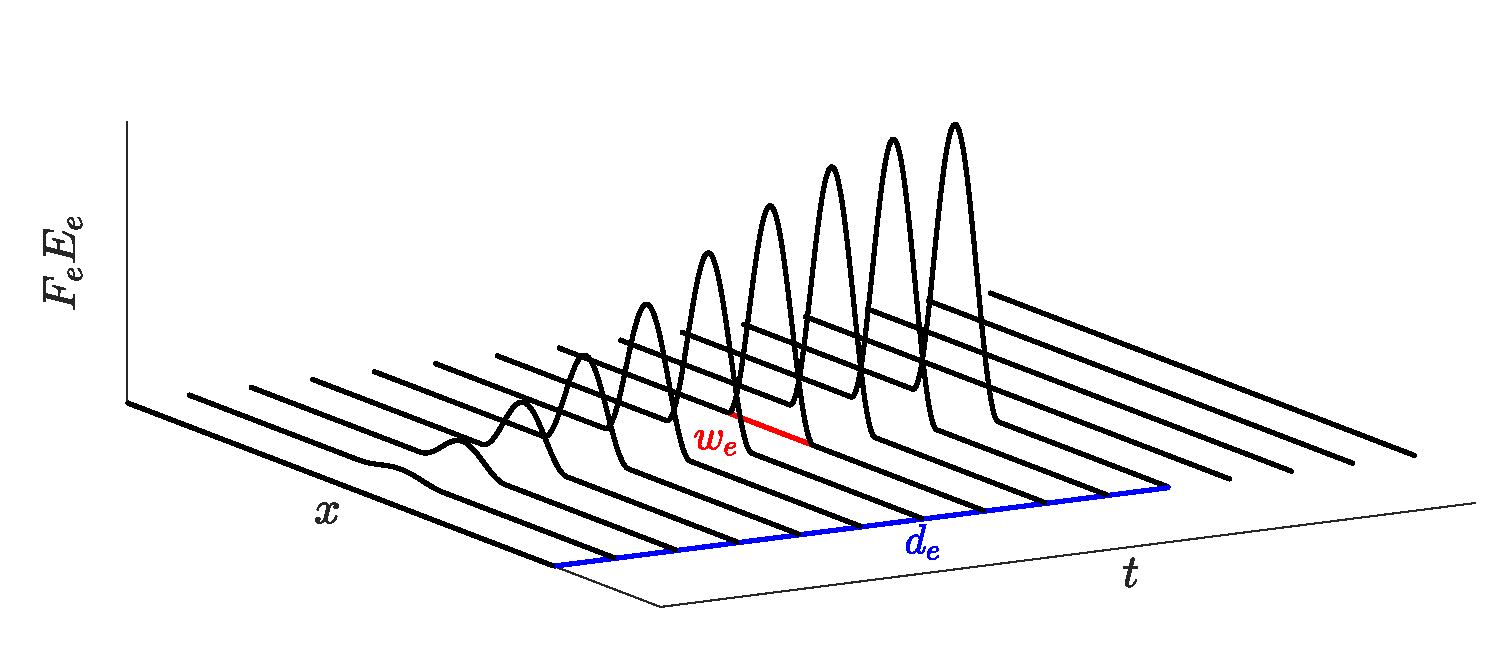
\includegraphics[width=1.0\columnwidth]{excitation.eps}
\caption{A visualisation of the excitation used in our implementation presented in Equation \eqref{eq:excitedString}. The location of excitation $x_\text{e}$ is shown in green, excitation width $w_\text{e}$ in red and excitation duration $d_\text{e}$ in blue (also see Equations \eqref{eq:distribution} and \eqref{eq:excitation}). \label{fig:exctiation}}
\end{figure}

\subsubsection{Pitch}
There are several ways to change the pitch of the string
According to \cite{Bilbao2009:NumericalSoundSynthesis},  the fundamental frequency can be approximately calculated using

\begin{equation}
    f_0 \approx \frac{\gamma}{2}.
\end{equation}

However, as the grid spacing $h$ is dependent on $\gamma$ according to the condition found in \eqref{eq:stabilityString}, we must put a lower limit on the number of points $N$ if we plan to dynamically increase $\gamma$.

%maybe it would be better to move the boundary to a different gridpoint and use interpolation for determination of the values around the boundary
Another way to generate different pitches is to add damping to the model at specific points that acts as a fretting finger. The advantage of this is that the condition \eqref{eq:stabilityString} will never be violated. On top of this, a tapping sound will be introduced when fretting the string, making it more realistic than changing the wave speed. If the string is fretted st single location $x_\text{f} \in [0, 1]$ and $l_\text{f} = \text{floor}(x_\text{f}/h)$ we use
\begin{equation}
u_l^n = 
    \begin{cases}
        \hfil 0, & l = l_\text{f} - 1 \vee l = l_\text{f}\\
        \hfil (1-\alpha_\text{f}^\epsilon) u_l^n, & l = l_\text{f} + 1\\
        \hfil u_l^n, & \text{otherwise}
    \end{cases}
\end{equation}
where $\alpha_\text{f} = x_\text{f}/h - l_\text{f}$ describes the fractional location of $x_\text{f}$ between two grid points. The disadvantage of using this technique over changing the wave speed $\gamma$ is that the effect of damping between grid points does not linearly scale to pitch. We thus added $\epsilon = 7$ as a heuristic value to more properly map finger position to pitch.

\subsection{Plate}
We chose the number of points to be $N_x = 20$ and $N_y = 10$ as this was found to be a great speed/quality tradeoff.

An interesting parameter to change is the plate stiffness $\kappa$. 

\subsection{Connections}
As mentioned before, the connections need to be calculated using 

In order to calculate the connection forces $F_\alpha$ and $F_\beta$, the relative displacement of the connection points $E_\alpha$ and $E_\beta$ is needed. We must thus have knowledge of the states of connected elements $\alpha$ and $\beta$. 

\subsection{Sensel Morph}
The Sensel Morph (or further referred to as Sensel) is an expressive touch controller that senses position and force of objects
\subsubsection{Mapping strategies}
Something about the different prototype mappings, and the "final" mapping 

\section{Instruments and User Interaction}\label{sec:instruments}
In this section, several configurations of strings, plates and connections that are inspired by real-life instruments will be presented. We subdivide string-elements into three types: bowed, plucked and sympathetic strings. All strings will be connected to one plate which simulates an instrument body. The user can control the plate stiffness and increase it to generate more interaction between the strings. Furthermore, the user can change the output level of each element type. Apart from these parameters, which are controlled by the mouse, the instruments are fully controlled by two Sensels. The instruments we have chosen as our inspiration are the sitar, the hammered dulcimer and the hurdy gurdy. Videos and sound examples can be found through the following link:...

\subsection{User interface}
Strings are shown as coloured paths (also see figures in this section). The state $u$ of the model is visualised using the vertical displacement of the paths. Bowed strings are shown in cyan on the top left. The bow is shown as a yellow rectangle and moves on interaction. The fretting position is shown as a yellow circle. Plucked strings are shown in purple i the top right, underneath which the sympathetic strings are shown in light green. The plate is shown in the bottom using a 18x8 grid of rectangles (clamped gridpoints are not shown). Its state is visualised using a grey-scale.

Furthermore, connections are shown using orange circles/squares for the points of connection and dotted lines between connected elements.

Lastly, all parameters that are controlled by the mouse - output-mix, plate stiffness, etc - are located in a column on the right side of the UI.

\subsection{Bowed Sitar}
The sitar is originally an Indian string instrument that has both fretted strings and sympathetic strings. Instead of picking the fretted strings, we extended the model to bow these strings. Our implementation consists of 2 bowed strings, 13 sympathetic strings and 5 plucked strings (as it is also possible to strum the sympathetic strings). See Figure \ref{fig:bowedSitar} for a visual of the implementation. One Sensel is vertically subdivided into two sections, one for each bowed string, The first finger registered by the Sensel is mapped to the bow and the second is mapped to a fretting finger on the string controlling pitch. The frets are not implemented as such (the pitch is continuous), but they are visualised for reference. The horizontal position of the first finger is mapped to the bowing position on the string, the vertical velocity  to the bow velocity with a maximum of $v_\text{B} = 0.2$ m/s and the finger force is linked to the excitation function with a maximum of $F_\text{B} = 100$ m/s$^2$. The other Sensel is subdivided into 5 sections mapped to the plucked strings. 

\begin{figure}[h]
\centering
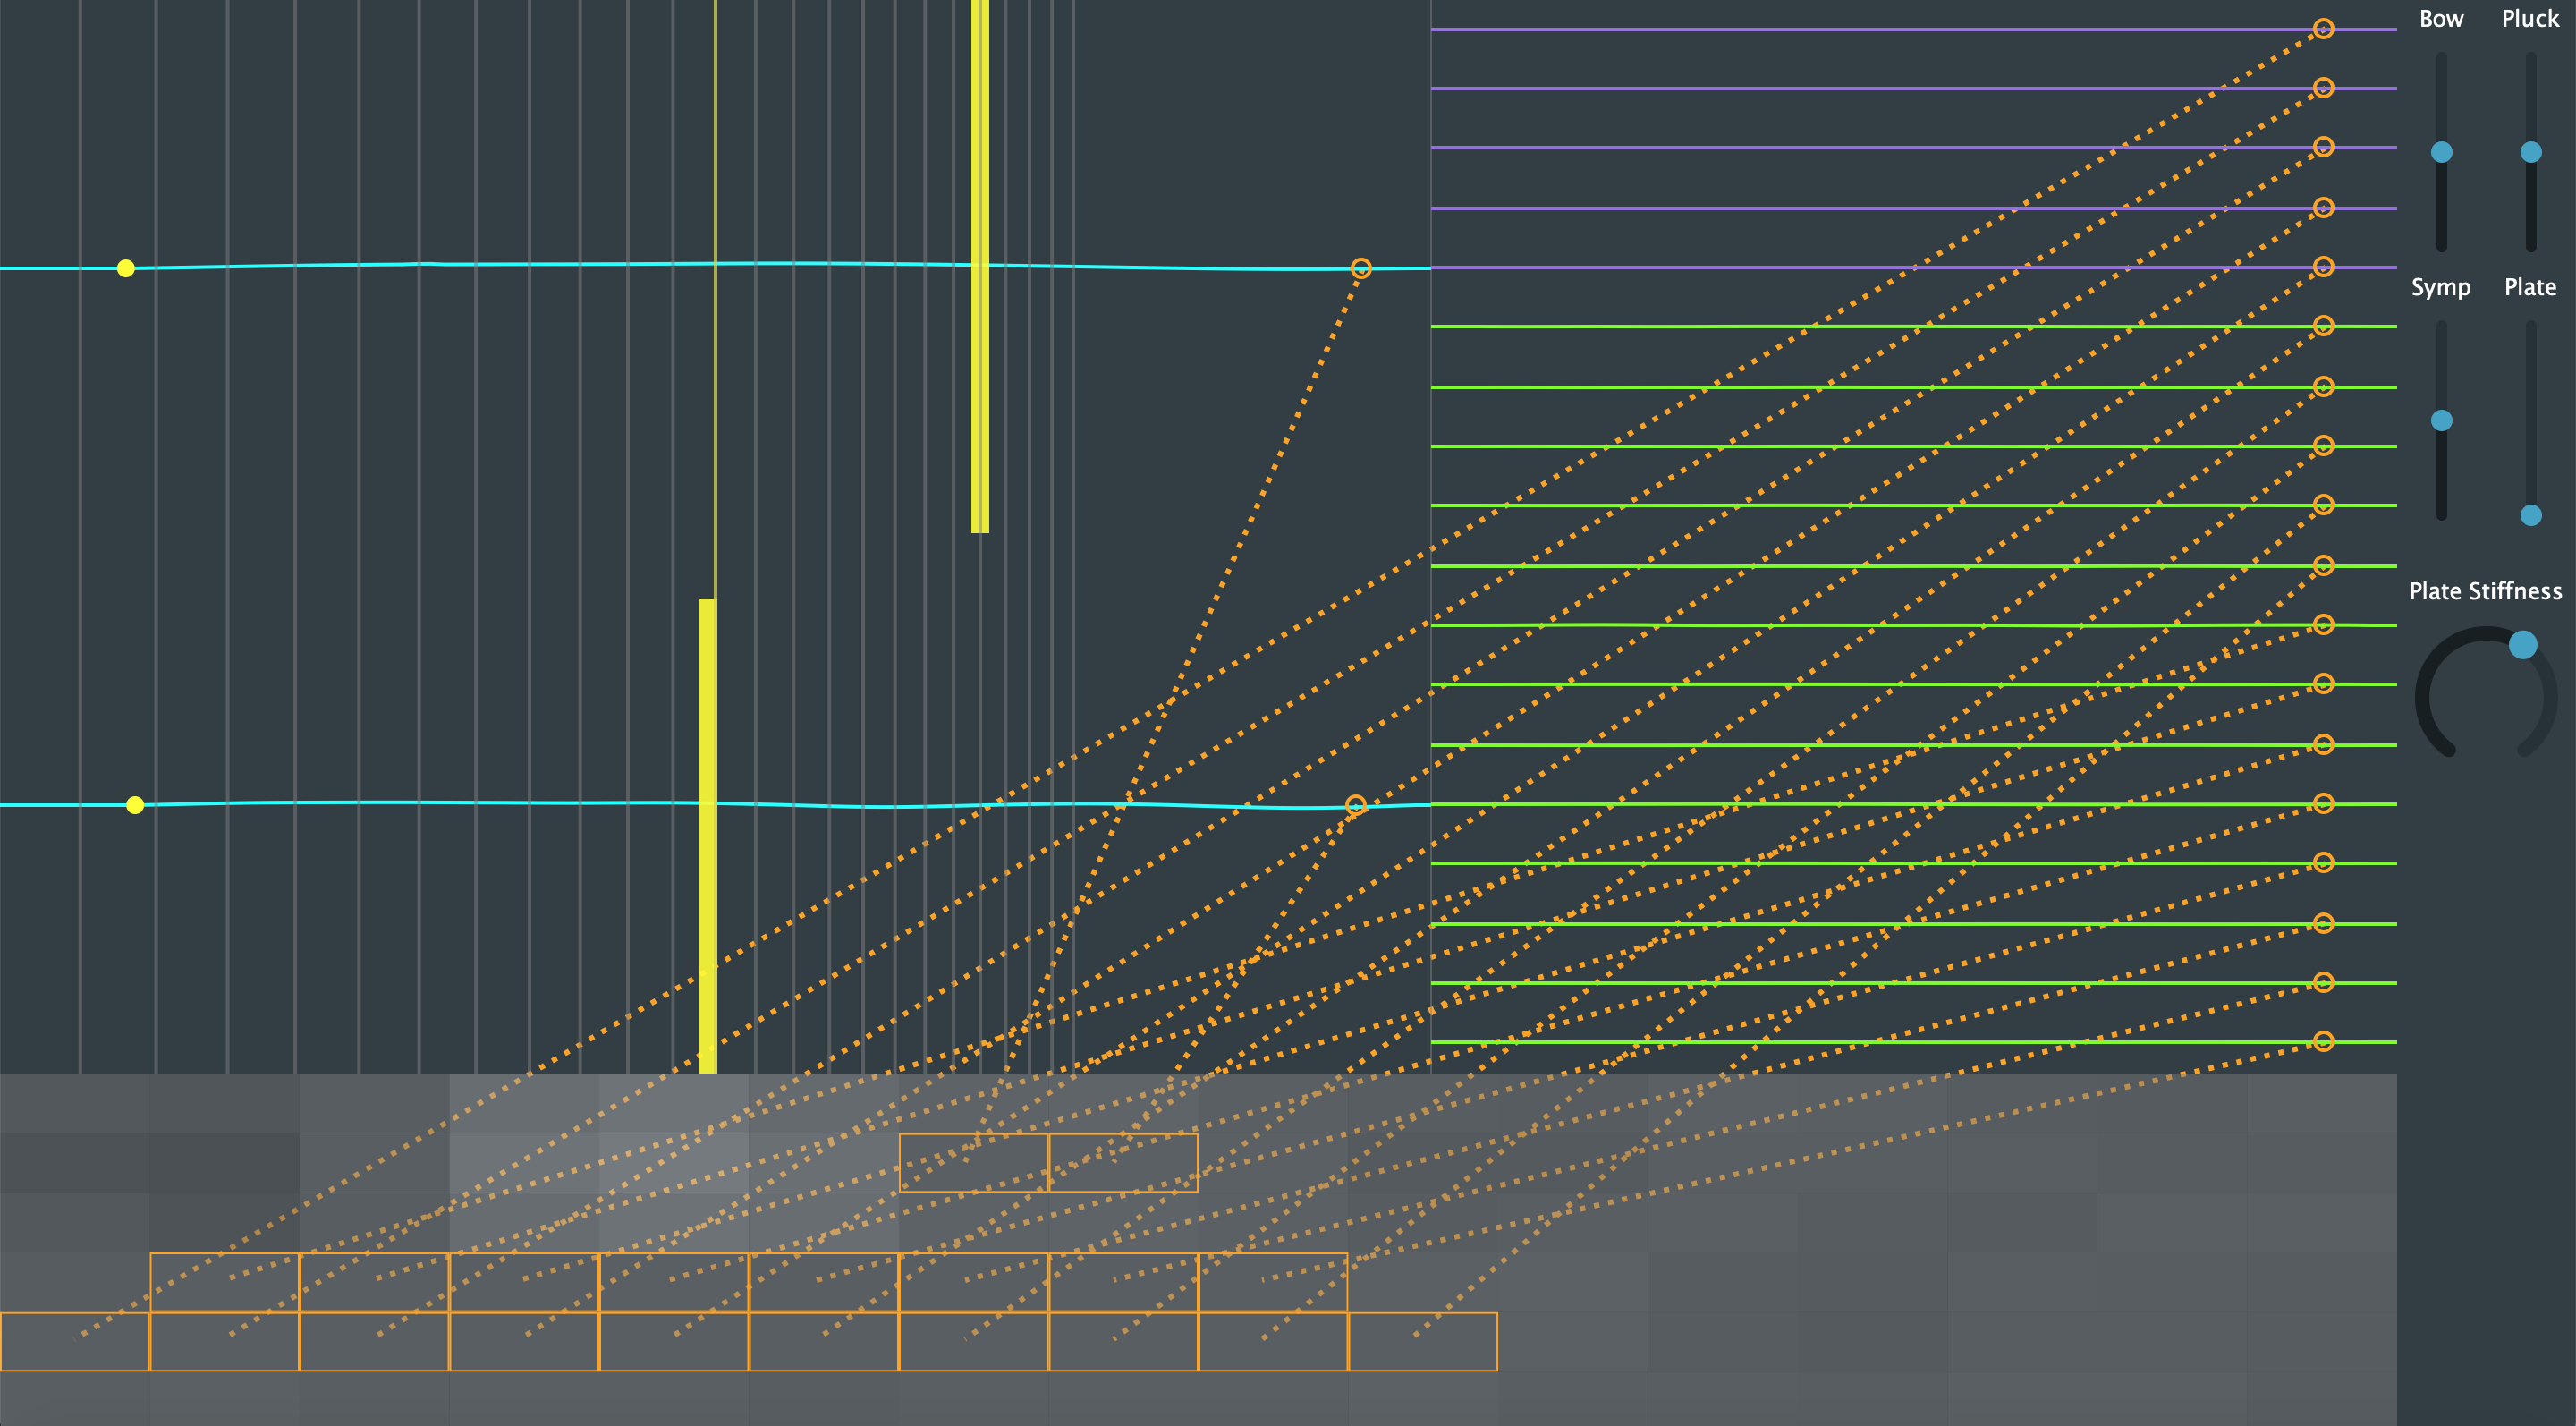
\includegraphics[width=1.0\columnwidth]{LATEX/BowedSitar.png}
\caption{The bowed sitar application. The descriptions of the different elements and other objects are shown in the image, but will (naturally) not be visible in the application. \label{fig:bowedSitar}}
\end{figure}

\subsection{Hammered Dulcimer}
The hammered dulcimer is an instrument that can be seen as an 'open piano' where the musician has the hammers in their hand. Just like the piano, the strings are grouped in pairs or triples %triplets?
that are played simultaneously. 
In our implementation, we have 20 pairs of plucked strings. The excitation (which are plucked strings with a longer excitation length) %need to work on a hammer model 
One of each pair is connected to the plate which slightly detunes it 

\subsection{Hurdy Gurdy}
The hurdy gurdy is an instrument that consists of bowed and sympathetic strings. The bowing happens through a rosined wheel attached to a crank and bows these strings as the crank is turned. It is possible to change the pitch of a few bowed strings - the melody strings - using buttons that press tangent pins on the strings at different positions. The other strings, referred to as drone strings, are mostly tuned lower than the melody strings and provide the base notes of the instrument. The musician can place the bowed strings on rests that keep the wheel from interacting with it. 

Our implementation consists of 5 bowed strings subdivided into 2 drone strings tuned to A2, E3 and 3 melody strings tuned to A3, E4 and A4 and 13 sympathetic strings. 

The Sensel is vertically subdivided into 5 rows that control whether the strings are placed on the wheel. The bowing velocity is mapped to the average pressure of the fingers. The pitch (in the model this is the wave-speed $\gamma$) of the melody-strings are changed by a midi controller.


\section{Discussion}\label{sec:discussion}

Body should not be plate.
We did an informal test with a lecturer of the Rytmisk Center København 
The interaction with the bow has been found very natural. Bow force and velocity... 

\section{Conclusion and Future Work}\label{sec:conclusion}
Speed up more: AVX vector / GPU / multithreading such as \cite{Webb2015}

Model instrument bodies


\begin{acknowledgments}
We would like to thank Stefan Bilbao for his guidance during the course of this project. 
\end{acknowledgments} 

%%%%%%%%%%%%%%%%%%%%%%%%%%%%%%%%%%%%%%%%%%%%%%%%%%%%%%%%%%%%%%%%%%%%%%%%%%%%%
%bibliography here
\bibliography{smc2019bib}
\end{document}
